\section{Accelerating Text Classifier}

\subsection{Acheived Performance}

\begin{figure}[h]
    \centering
    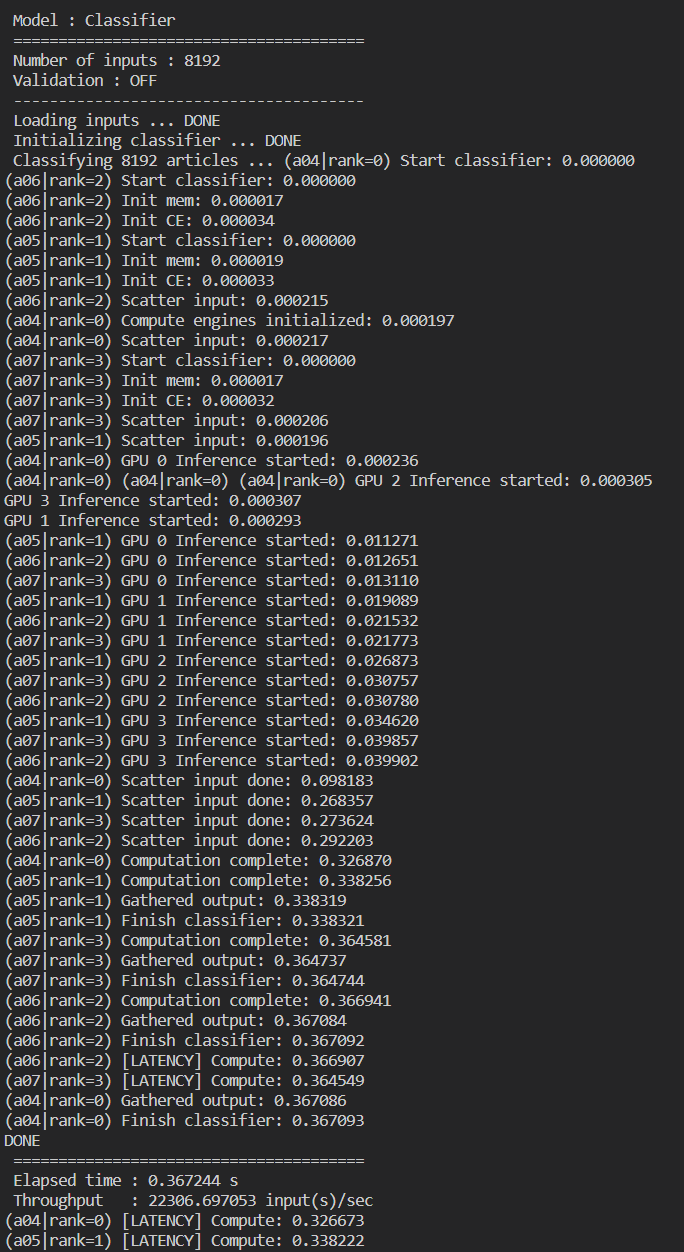
\includegraphics[width=0.6\textwidth]{imgs/best_record.png}
    \caption{The best record of my implementation.}
    \label{fig:best_record}
\end{figure}

총 8192개의 input을 4개 노드에서 연산하도록 하여 최고 
\textbf{9399.12 input(s)/sec}의 성능을 달성하였다[Fig.~\ref{fig:best_record}].

\subsection{Implementation}
Root 노드는 MPI를 이용하여 나머지 노드에 input을 분배한다.
각 노드는 여러 input을 batch로 묶어 처리하며,
classifier의 모든 연산을 GPU에서 수행하고 최종 결과만을 CPU로 전송한다.
다음 섹션에서 설명할 기법들을 사용하여 연산에 걸리는 시간을 매우 줄일 수 있었으며,
이로 인해 8192개의 input을 네 노드에 분산하는 데 걸리는 시간인
약 0.8초 정도의 시간보다 훨씬 적은 시간이 걸리게 되었다.
이에 MPI로 input을 분산하는 과정을 fine-grained하게 쪼개어 compute와 interleave되도록 하였다.

그 결과, 제출한 classifier의 성능은 \textbf{완전히 network-bound}가 되었다고 할 수 있으며,
이는 8192개의 input을 4개의 노드에서 처리하는 데 필요한 \textbf{최소한의 시간을 사용}하였음을 의미한다.
따라서 \textbf{같은 환경에서 얻을 수 있는 최고 성능을 달성}하였다고 할 수 있다.

마지막 input 분산 이후 마지막 연산에 걸리는 시간이나, 이외 자잘한 부분에서 소요되는 시간은
input을 분산하는 시간에 비해 매우 작으며, 이는 무시할 수 있는 수준이다.
또한, 앞서 말한 바와 같이 제출한 classifier의 성능은 완전한 network-bound가 되었으므로,
slurm에 의해 배정되는 노드의 종류나 그 사이의 네트워크 topology등의 요인으로
\textbf{측정하는 순간의 서버 클러스터의 네트워크 환경에 따라 약간의 편차가 있을 수 있다.}
하지만 대부분의 경우 9000 input(s)/sec 이상의 성능을 얻을 수 있었으며,
반복을 통해 얻은 최고 성능은 9399.12 input(s)/sec이었다.
\textbf{최종 성능 채점시에 이와 같은 점이 충분히 고려되어야 한다.}

\subsection{Latency Breakdown}

자체 구현한 디버그 모드로 실행하여 Tab.~\ref{tab:latency_breakdown}과 같이 
latency를 세부적으로 분석하였다. 단위는 초(sec)이다.
측정시에 전체 소요시간은 0.880531 sec 이었으며, throughput은 9303.474877 input(s)/sec 이었다.

\begin{table}[]
    \centering
    \begin{tabular}{l|rrrr}
    \multicolumn{1}{c|}{NODE} & \multicolumn{1}{c}{00(root)} & \multicolumn{1}{c}{01} & \multicolumn{1}{c}{02} & \multicolumn{1}{c}{03} \\ \hline
    Classifier 시작           & 0.000000               & 0.000000               & 0.000000               & 0.000000               \\
    메모리 초기화              & 0.000000               & 0.000016               & 0.000029               & 0.000013               \\
    Compute Engine 초기화     & 0.000183               & 0.000032               & 0.000065               & 0.000026               \\
    Input 분산 시작            & 0.000206               & 0.000215               & 0.000296               & 0.000199               \\
    GPU0 연산 시작             & 0.000225               & 0.005239               & 0.009069               & 0.013125               \\
    GPU1 연산 시작             & 0.000331               & 0.017486               & 0.021290               & 0.025264               \\
    GPU2 연산 시작             & 0.000374               & 0.029747               & 0.033609               & 0.037557               \\
    GPU3 연산 시작             & 0.000270               & 0.041901               & 0.045766               & 0.049682               \\
    Input 분산 종료            & 0.810448               & 0.802368               & 0.806489               & 0.810455               \\
    Compute Engine 종료       & 0.810464               & 0.826805               & 0.831194               & 0.835908               \\
    Output을 root에 전달       & 0.836118               & 0.826890               & 0.836094               & 0.836072               \\
    Classifier 종료           & 0.836125               & 0.826905               & 0.836106               & 0.836081              
    \end{tabular}
    \caption{Latency breakdown of my implementation, in seconds.}
    \label{tab:latency_breakdown}
\end{table}

\subsection{Optimization Techniques}

다음과 같은 최적화 기법을 나열한 뒤, 하나씩 적용하며 최적화하였다.

\begin{itemize}
    \item Synchronously offload input to other nodes using MPI

    \item Asynchronously offload input to other nodes using MPI

    \item Calculate multiple batches at once

    \item Calculate each operators with CUDA: \texttt{conv1d}, \texttt{layernorm}, \texttt{relu}, \texttt{maxpool1d}, \texttt{linear}, etc.
        
    \item Store most of intermediate features in global memory
    
    \item Create weakly fused operators: \texttt{conv1d\_relu}, \texttt{conv1d\_stat}, \texttt{linear\_relu}, etc.

\end{itemize}

\subsection{Optimization History}

다음과 같은 순서로 최적화를 진행하였으며, 그 각 과정에서 얻은 성능을 측정하였다.

\begin{enumerate}
    \item Baseline: 2.12 input(s)/sec
    \item Synchronous offload: 8.33 input(s)/sec
    \item Naively batched computation: 7.86 input(s)/sec
    \item Naive CUDA conv1d: 12.76 input(s)/sec
    \item Replace every conv1d with \texttt{conv1d\_cuda}, fuse \texttt{relu}: 165.00 input(s)/sec
    \item Use multiple GPUs: 555.00 input(s)/sec
    \item Naive CUDA linear: 727.20 input(s)/sec
    \item Replace every linear with \texttt{linear\_cuda}, fuse \texttt{relu}: 1152.75 input(s)/sec
    \item Merged maxpool1d and relu: 1290.74 input(s)/sec
    \item \texttt{conv1d\_k3} square blocking: 1505.14 input(s)/sec
    \item \texttt{conv1d\_k3} rectangular blocking: 1550.79 input(s)/sec
    \item \texttt{conv1d} hyperparameter tuning: 2537.34 input(s)/sec
    \item \texttt{conv1d\_k7} rectangular blocking: 3013.50 input(s)/sec
    \item Batched processing: 3501.90 input(s)/sec
    \item linear rectangular: 3644.37 input(s)/sec
    \item \texttt{conv1d\_k3}, \texttt{conv1d\_k7} avoid bank conflict: 3753.42 input(s)/sec
    \item Naive linear normalization: 4241.36 input(s)/sec
    \item Naive maxpool1d: 5266.67 input(s)/sec
    \item Memory cleanup: 5865.32 input(s)/sec
    \item No more Tensor type: 6175.81 input(s)/sec
    \item Scatter into Scatterv: 5924.65 input(s)/sec
    \item Networking \& offloading interleaved: 8587.53 input(s)/sec
    \item Fine-grained interleaving: \textbf{9399.12 input(s)/sec}
\end{enumerate}
